
\documentclass{article}
\usepackage[utf8]{inputenc}
\usepackage{mathtext}
\usepackage{amsmath}
\usepackage[colorlinks=true, linkcolor=blue]{hyperref}
\usepackage[T1]{fontenc}
\usepackage[utf8]{inputenc}
\usepackage[english, bulgarian, russian]{babel}
\usepackage{tikz}
\usepackage{pgfplots}
\usepackage{indentfirst}
\usepackage[export]{adjustbox}
\usepackage{lipsum} % sample text
\usepackage{floatflt}
\usepackage{multirow}
\usepackage{geometry} \geometry{verbose,a4paper,tmargin=2cm,bmargin=2cm,lmargin=1.5cm,rmargin=1.5cm}
\setlength{\parindent}{0.65cm}
\setlength{\parskip}{0.15cm}

\usepackage{wrapfig}
\usepackage{array,graphicx,caption}


%Матеша
\usepackage{amsmath,amsfonts,amssymb,amsthm,mathtools,  mathrsfs, wasysym} % AMS
\usepackage{icomma} % "Умная" запятая

%\mathtoolsset{showonlyrefs=true} % Показывать номера только у тех формул, на которые есть \eqref{} в тексте.

%% Шрифты
\usepackage{euscript}	 % Шрифт Евклид
\usepackage{mathrsfs} % Красивый матшрифт

%% Свои команды
\DeclareMathOperator{\sgn}{\mathop{sgn}}

%% Перенос знаков в формулах (по Львовскому)
\newcommand*{\hm}[1]{#1\nobreak\discretionary{}
	{\hbox{$\mathsurround=0pt #1$}}{}}


% Рисунки
\usepackage{subcaption,floatrow,graphicx,calc}
\usepackage{wrapfig}

% Создаёем новый разделитель
\DeclareFloatSeparators{mysep}{\hspace{1cm}}



 
\begin{document}
\def\figurename{Рисунок}
\begin{titlepage}
\begin{center}
    {\large МОСКОВСКИЙ ФИЗИКО-ТЕХНИЧЕСКИЙ ИНСТИТУТ (НАЦИОНАЛЬНЫЙ ИССЛЕДОВАТЕЛЬСКИЙ УНИВЕРСИТЕТ)}
\end{center}
\begin{center}
    {\largeФизтех-школа биологической и медицинской физики}
\end{center}

\vspace{1cm}
{\huge
\begin{center}
    {\bf Лабораторная работа по общей физике}\\
    \vspace{0.5cm}
    5.4.2 Исследование энергетического спектра $\beta$-частиц и определение их максимальной энергии при помощи магнитного спектрометра.
\end{center}
}

\vspace{4cm}
\begin{flushright}
{\LARGE Выполнили студенты группы Б06-103:\\ Фитэль Алена \\Флоренская Лидия\\}

\end{flushright}
\vspace{9cm}
\begin{center}
    Долгопрудный, 2023 г.
\end{center}
\end{titlepage}

\newpage
	\textbf{Цель работы:} измерить пробег $\alpha$-частиц в воздухе двумя способами: с помощью торцевого счетчика Гейгера и синтиляционного счетчика, -- по полученным данным определить энергию частиц.

\section{Теоретическое введение}
	При $\alpha$-распаде исходное родительское ядро испускает ядро гелия и превращается в дочернее ядро, число протонов и число протонов уменьшается на две единицы. Функциональная свзязь между энергией $\alpha$-частицы $E$ и периодом полураспада радиоактивного ядра $T_{1/2}$:
	\begin{equation*}
		 \lg T_{1/2} = \frac{a}{\sqrt{E}} + b.
	\end{equation*}
	
	Для описания связи между энергией $\alpha$-частицы и ее пробегом пользуются эмпирическими соотношениями. В диапазоне энергий $\alpha$-частиц от 4 до 9 МэВ эта связь хорошо описывается выражением:
	\begin{equation*}
		\label{eq:R(E)}
		\tag{$\star$}
		R = 0,32E^{3/2}
	\end{equation*}
	

\section{Экспериментальная установка}
		В данной работе в качестве источника $\alpha$-частиц используется ${239}$Pu с периодом полураспада $T_{1/2} = 2,44 \cdot 10^4$ лет. Альфа-частицы, испускаемые ${239}$Pu состоят их трех моноэнергетических групп, различие между которыми лежит в пределах 50 кэВ. При той точности, которая достигается в наших опытах, их можно считать совпадающими по энергии, равной 5,15 МэВ.
 
 Пробег $\alpha$-частиц в воздухе будем определяеть треями способами:
	\begin{enumerate}
		\item
			С помощью счетчика Гейгера -- рис.~\ref{pic1};
		\item
			C помощью сцинтилляционного счетчика -- рис.~\ref{pic2};
		\item
			C помощью ионизационной камеры -- рис.~\ref{pic3}.
	\end{enumerate} 
	
	\thisfloatsetup{floatrowsep=mysep}	
	\begin{figure}[h!]
		\ffigbox{
			\begin{subfloatrow}[3]
				\ffigbox[\FBwidth]{\caption{}}%
				{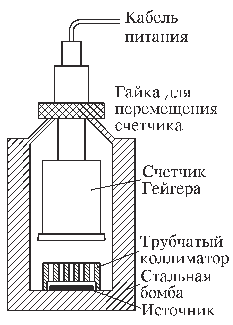
\includegraphics[scale=1]{ustanovka1.pdf}{\label{pic1}}}
				\ffigbox[\FBwidth]{\caption{}}%
				{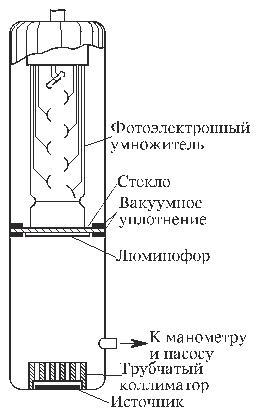
\includegraphics[scale=0.8]{ustanovka2.pdf}{\label{pic2}}}
				\ffigbox[\FBwidth]{\caption{}}%
				{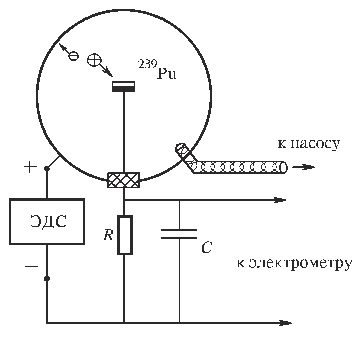
\includegraphics[scale=1]{ustanovka3.pdf}{\label{pic3}}}          
			\end{subfloatrow}
		}
		{\caption{Экспериментальные установки: (a) - cчетчик Гейгера, (b) - сцинтилляционный счетчик, (с) - ионизационная камера.}}
	\end{figure}
	

	
\subsection{Счётчик Гейгера}

    Для определения пробега $\alpha$-частиц с помощью счетчика радиоактивный источник помещается на дно стальной цилиндрической бомбы, в которой может перемещаться торцевой счетчик Гейгера. Его чувствительный объем отделен от наружной среды тонким слюдяным
    окошком, сквозь которое могут проходить $\alpha$-частицы.


    Импульсы, возникающие в счетчике, усиливаются и регистрируются пересчетной схемой. Путь частиц в воздухе зависит от расстояния
    между источником и счетчиком. Перемещение счетчика производится путем вращения гайки, находящейся на крышке бомбы. Расстояние
    между счетчиком и препаратом измеряется по шкале, нанесенной на держатель счетчика.



\subsection{Сцинтилляционный счётчик}

    Установка состоит из цилиндрической камеры, на дне которой находится исследуемый препарат. Камера герметично закрыта стеклянной пластинкой, на которую с внутренней стороны нанесен слой люминофора. С наружной стороны к стеклу прижат фотокатод фотоумножителя. Оптический контакт ФЭУ-стекло обеспечивается тонким слоем вазелинового масла.
        
    
    Сигналы с фотоумножителя через усилитель поступают на пересчетную установку. Расстояние между препаратом и люминофором составляет 9 см, так что $\alpha$-частицы не могут достигнуть люминофора при обычном давлении. Определение пробега сводится к измерению зависимости интенсивности счета от давления в камере.


    
\subsection{Иниозационная камера}

    Ионизационная камера -- прибор для количественного измерения ионизации, произведенной заряженными частицами при прохождении
    через газ. Камера представляет собой наполненный газом сосуд с двумя электродами. Сферическая стенка прибора служит одним из электродов, второй электрод вводится в газ через изолирующую пробку. К электродам подводится постоянное напряжение от источника ЭДС.
    Заполняющий сосуд газ сам по себе не проводит электрический ток, возникает он только при прохождении быстрой заряженной частицы, которая
    рождает в газе на своем пути ионы.

    Поместим на торец внутреннего электрода источник ионизирующего излучения, заполним объем камеры воздухом. Зависимость силы тока, протекающего через камеру, от приложенной разности потенциалов представлен на рисунке. Плато в зависимости объясняется отсутствием рекомбинации ионов на своём пути, то есть ионы доходят до противоположного электрода.

    Прохождение тока через камеру регистрируется посредством измерения напряжения на включенном в цепь камеры сопротивлении $R$. При изменении давления в камере ионизационный ток меняется так, как это показано на рисунке. При небольших давлениях газа $\alpha$-частицы передают часть энергии стенкам камеры. По достижении давления $P_0$ все они заканчивают свой пробег внутри газа, и дальнейшее возрастание тока прекращается. Для определения давления $P_0$ чаще всего пользуются методом экстраполяции, продолжая наклонный и горизонтальный участки кривой до пересечения. Найденный таким образом пробег затем должен быть приведен к нормальному давлению и температуре 15 $^\circ C$.


\section{Ход работы}




\subsection{Исследование пробега $\alpha$-частиц с помощью счетчика Гейгера}
	
Проведем измерение зависимости скорости счета $N$ от расстояния $x$ между источником и счетчиком(Таблица % \caption{Зависимость скорости счета от расстояния}
			% \label{AlphaParticles_N(x)}). 

\\
Построим график $N(x)$. Найдем значения $R_\text{э}$ и $R_\text{ср}$:
   \begin{enumerate}
   \item  Аппроксимируем полученный набор точек сигмоидой:
\[N(x) = \frac{A}{1 + \exp{\left(\frac{x - x_0}{B}\right)}} + C \]
 \[A = (14,7 \pm 0,2) \hspace{1 cm } B = (0,46 \pm 0,04) \text{ мм} \hspace{1 cm } C = (0,26 \pm 0,03) \hspace{1 cm } x_0 = (17,7 \pm 0,5) \text{ мм} \]

 
\item Проведем аппроксимацию центральной части графика 	$N(x)$ линейной прямой:
\[ N = ax + b\]
\[a = \hspace{1 cm } b = \]

\item Из графиков получаем:
		\begin{itemize}
			\item $R_\text{ср} = x_0 = (17,7 \pm 0,5) \text{ мм} = (1,77 \pm 0,05) \text{ см}$ - из сигмоиды;
			
			
			\item $R_\text{э} \,\, = (19 \pm 3) \text{ мм} = (1,9 \pm 0,3) \text{ см}$ - из линейной аппроксимации (точка пересечения с осью абцисс).
		\end{itemize}

  
\end{enumerate}
При плотности воздуха $\rho = 1,17 \cdot 10^{-3} \;\dfrac{\text{г}}{\text{см}^3}$ ($P = 99,3 \text{ кПа}$, $t = 22\;^\circ \text{C}$):
		\begin{itemize}
			\item $R'_\text{ср} = (2,07 \pm 0,06) \cdot 10^{-3} \;\dfrac{\text{г}}{\text{см}^2}$;
			
			
			\item $R'_\text{э} \,\, = (2,2 \pm 0,4) \cdot 10^{-3} \;\dfrac{\text{г}}{\text{см}^2}$.
		\end{itemize}
	
		Соответствующая энергия:
		\begin{itemize}
			\item $E_\text{ср} = (3,13 \pm 0,06) \text{ МэВ}$;
			
			\item $E_\text{э} \,\, = (3,3 \pm 0,4) \text{ МэВ}$.
		\end{itemize}
	
	Как видим, результаты совпадают по порядку с истинным значением $E = 5,15$ МэВ. Расхождение объясняется  тем, что часть энергии $\alpha$-частиц тратится на преодоление слюдяной пластинки.

% Please add the following required packages to your document preamble:
% \usepackage{multirow}
\begin{table}[h!]
\centering
\begin{tabular}{|r|c|r|r|r|r|r|}
\hline
\multicolumn{1}{|l|}{$x$, мм} &
  \multicolumn{1}{l|}{$\sigma_x$, мм} &
  \multicolumn{1}{l|}{$N_0$} &
  \multicolumn{1}{l|}{$t$, с} &
  \multicolumn{1}{l|}{$N$, с$^{-1}$} &
  \multicolumn{1}{l|}{$\sigma_{N}$, с$^{-1}$} &
  \multicolumn{1}{l|}{$\epsilon(N),   \%$} \\ \hline
40.00 & \multirow{18}{*}{0.25} & 19  & 107 & 0.18 & 0.04 & 21 \\ \cline{1-1} \cline{3-7} 
35.00 &                        & 38  & 213 & 0.18 & 0.03 & 16 \\ \cline{1-1} \cline{3-7} 
30.00 &                        & 26  & 185 & 0.14 & 0.03 & 19 \\ \cline{1-1} \cline{3-7} 
25.00 &                        & 36  & 219 & 0.16 & 0.03 & 17 \\ \cline{1-1} \cline{3-7} 
20.00 &                        & 30  & 121 & 0.25 & 0.04 & 17 \\ \cline{1-1} \cline{3-7} 
15.00 &                        & 24  & 156 & 0.15 & 0.03 & 21 \\ \cline{1-1} \cline{3-7} 
10.00 &                        & 30  & 78  & 0.38 & 0.06 & 17 \\ \cline{1-1} \cline{3-7} 
5.00  &                        & 202 & 13  & 15.5 & 1.1  & 7  \\ \cline{1-1} \cline{3-7} 
0.00  &                        & 201 & 14  & 14.4 & 1.0  & 7  \\ \cline{1-1} \cline{3-7} 
2.00  &                        & 639 & 45  & 14.2 & 0.6  & 4  \\ \cline{1-1} \cline{3-7} 
1.25  &                        & 327 & 20  & 16.4 & 0.9  & 6  \\ \cline{1-1} \cline{3-7} 
3.75  &                        & 322 & 21  & 15.3 & 0.9  & 6  \\ \cline{1-1} \cline{3-7} 
6.25  &                        & 549 & 39  & 14.1 & 0.6  & 4  \\ \cline{1-1} \cline{3-7} 
7.00  &                        & 340 & 27  & 12.6 & 0.7  & 5  \\ \cline{1-1} \cline{3-7} 
8.00  &                        & 189 & 21  & 9.0    & 0.7  & 7  \\ \cline{1-1} \cline{3-7} 
9.00  &                        & 126 & 47  & 2.7  & 0.2  & 9  \\ \cline{1-1} \cline{3-7} 
8.50  &                        & 183 & 26  & 7.0    & 0.5  & 8  \\ \cline{1-1} \cline{3-7} 
7.50  &                        & 140 & 12  & 11.7 & 1.0  & 9  \\ \hline
\end{tabular}
\caption{Зависимость скорости счет $N$ от расстояния $x$.}
\label{tab:my-table}
\end{table}
 
 
 
 \begin{figure}[h!]
			\centering
			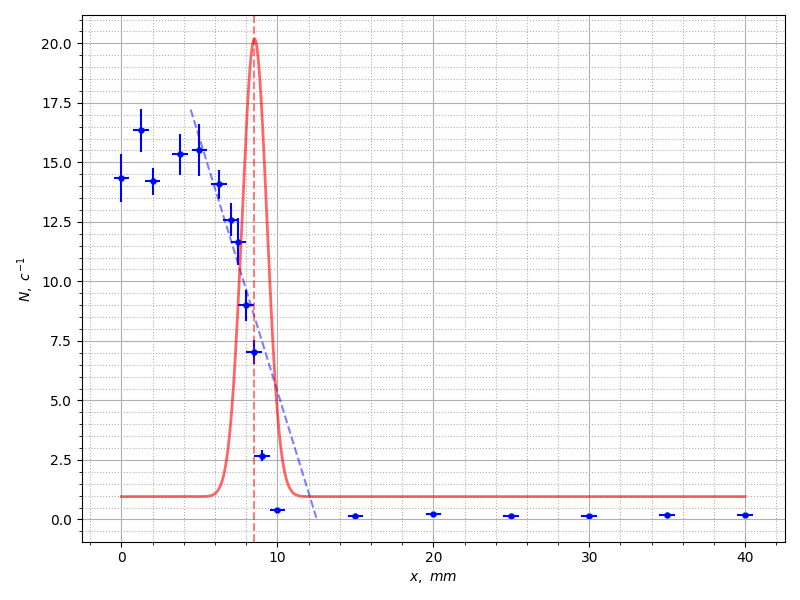
\includegraphics[width=0.9\linewidth]{5.4.1N(x).png}
			\caption{График зависимости $N(x)$}
   \end{figure}
		





	\subsection{Определение пробега $\alpha$-частиц с помощью сцинтилляционного счетчика}

Проведем измерение зависимости скорости счета $N$ от давления $p$ в камере(Таблица % \caption{Зависимость скорости счета от расстояния}
			% \label{AlphaParticles_N(x)}). 
\\
Построим график $N(p)$. Найдем значения $p_\text{э}$ и $p_\text{ср}$:
   \begin{enumerate}

   
   \item  Аппроксимируем полученный набор точек сигмоидой:
\[N(x) = \frac{A}{1 + \exp{\left(\frac{x - x_0}{B}\right)}} + C \]
 \[A = (14,7 \pm 0,2) \hspace{1 cm } B = (0,46 \pm 0,04) \text{ мм} \hspace{1 cm } C = (0,26 \pm 0,03) \hspace{1 cm } x_0 = (17,7 \pm 0,5) \text{ мм} \]

 
    \item Проведем аппроксимацию центральной части графика 	$N(x)$ линейной прямой:
\[ N = ax + b\]
\[a = \hspace{1 cm } b = \]

    \item Из графиков получаем:
		\begin{itemize}
			\item $p_\text{ср} = x_0 = (17,7 \pm 0,5) \text{ мм} = (1,77 \pm 0,05) \text{ см}$ - из сигмоиды;
			
			
			\item $p_\text{э} \,\, = (19 \pm 3) \text{ мм} = (1,9 \pm 0,3) \text{ см}$ - из линейной аппроксимации (точка пересечения с осью абцисс).
		\end{itemize}
    \end{enumerate}

Это давления, при которых длина свободного пробега равна расстоянию от источника для люминофора $L = 9$ см. 
		
		Пересчитаем длину свободного пробега для нормальных условий ($P = 760$ торр, $t = 15$ $^\circ$C):
		\begin{equation*}
			R_\text{э} = L\frac{P_\text{э}}{P_0}, 
		\end{equation*}
		\noindent где $P_0 = 760$ торр. Тогда:
		
		\begin{itemize}
			\item $R_\text{ср} = (1,32 \pm 0,05) \text{ см}$;
			
			
			\item $R_\text{э} \,\, = (2,4 \pm 0,2) \text{ см}$.
		\end{itemize}
		
		При плотности воздуха $\rho = 1,17 \cdot 10^{-3} \;\dfrac{\text{г}}{\text{см}^3}$ ($P = 99,3 \text{ кПа}$, $t = 22\;^\circ \text{C}$):
		\begin{itemize}
			\item $R'_\text{ср} = (1,55 \pm 0,06) \cdot 10^{-3} \;\dfrac{\text{г}}{\text{см}^2}$;
			
			
			\item $R'_\text{э} \,\, = (2,8 \pm 0,2) \cdot 10^{-3} \;\dfrac{\text{г}}{\text{см}^2}$.
		\end{itemize}
		
		Соответствующая энергия:
		\begin{itemize}
			\item $E_\text{ср} = (2,9 \pm 0,1) \text{ МэВ}$;
			
			\item $E_\text{э} \,\, = (3,8 \pm 0,2) \text{ МэВ}$.
		\end{itemize}
	
		Результаты совпадают по порядку с истинным значением. Однако они все еще не очень точны, хотя значение, полученное экстраполяцией, ближе этим методом, ближе всего к действительному значению. 

% Please add the following required packages to your document preamble:
% \usepackage{multirow}
\begin{table}[h!]
\centering
\begin{tabular}{|r|c|r|r|r|r|r|r|}
\hline
\multicolumn{1}{|l|}{$P_\text{изм}$, тор} &
  \multicolumn{1}{l|}{$\sigma_p$, бар} &
  \multicolumn{1}{l|}{$N_0$} &
  \multicolumn{1}{l|}{$P = P_0 - P_\text{изм}$, тор} &
  \multicolumn{1}{l|}{$t$, с} &
  \multicolumn{1}{l|}{$N$, с$^{-1}$} &
  \multicolumn{1}{l|}{$\sigma_{N}$, с$^{-1}$} &
  \multicolumn{1}{l|}{$\epsilon(N) \%,$} \\ \hline
0   & \multirow{20}{*}{\textit{5}} & 52   & 737 & 157 & 0.33 & 0.05 & 15   \\ \cline{1-1} \cline{3-8} 
720 &                              & 8111 & 17  & 21  & 386  & 4    & 1.04 \\ \cline{1-1} \cline{3-8} 
700 &                              & 9030 & 37  & 25  & 361  & 4    & 1.1  \\ \cline{1-1} \cline{3-8} 
680 &                              & 6594 & 57  & 20  & 330  & 4    & 1.2  \\ \cline{1-1} \cline{3-8} 
660 &                              & 5990 & 77  & 20  & 300  & 4    & 1.3  \\ \cline{1-1} \cline{3-8} 
640 &                              & 5419 & 97  & 20  & 271  & 4    & 1.5  \\ \cline{1-1} \cline{3-8} 
620 &                              & 4574 & 117 & 20  & 229  & 3    & 1.3  \\ \cline{1-1} \cline{3-8} 
600 &                              & 5442 & 137 & 30  & 181  & 2    & 1.1  \\ \cline{1-1} \cline{3-8} 
580 &                              & 2809 & 157 & 21  & 134  & 3    & 2    \\ \cline{1-1} \cline{3-8} 
560 &                              & 1931 & 177 & 20  & 97   & 2    & 2    \\ \cline{1-1} \cline{3-8} 
540 &                              & 1265 & 197 & 21  & 60.2 & 1.7  & 3    \\ \cline{1-1} \cline{3-8} 
520 &                              & 692  & 217 & 21  & 33   & 1.3  & 4    \\ \cline{1-1} \cline{3-8} 
500 &                              & 349  & 237 & 22  & 15.9 & 0.8  & 5    \\ \cline{1-1} \cline{3-8} 
480 &                              & 384  & 257 & 25  & 15.4 & 0.8  & 5    \\ \cline{1-1} \cline{3-8} 
460 &                              & 203  & 277 & 28  & 7.3  & 0.5  & 7    \\ \cline{1-1} \cline{3-8} 
440 &                              & 205  & 297 & 78  & 2.63 & 0.18 & 7    \\ \cline{1-1} \cline{3-8} 
400 &                              & 57   & 337 & 189 & 0.30 & 0.04 & 13   \\ \cline{1-1} \cline{3-8} 
350 &                              & 52   & 387 & 143 & 0.36 & 0.05 & 14   \\ \cline{1-1} \cline{3-8} 
300 &                              & 38   & 437 & 105 & 0.36 & 0.06 & 17   \\ \cline{1-1} \cline{3-8} 
200 &                              & 28   & 537 & 85  & 0.33 & 0.06 & 18   \\ \hline
\end{tabular}
\caption{Зависимость скорости счет $N$ от давления $p$.}
\label{tab:my-table}
\end{table}


 
    \begin{figure}[h!]
			\centering
			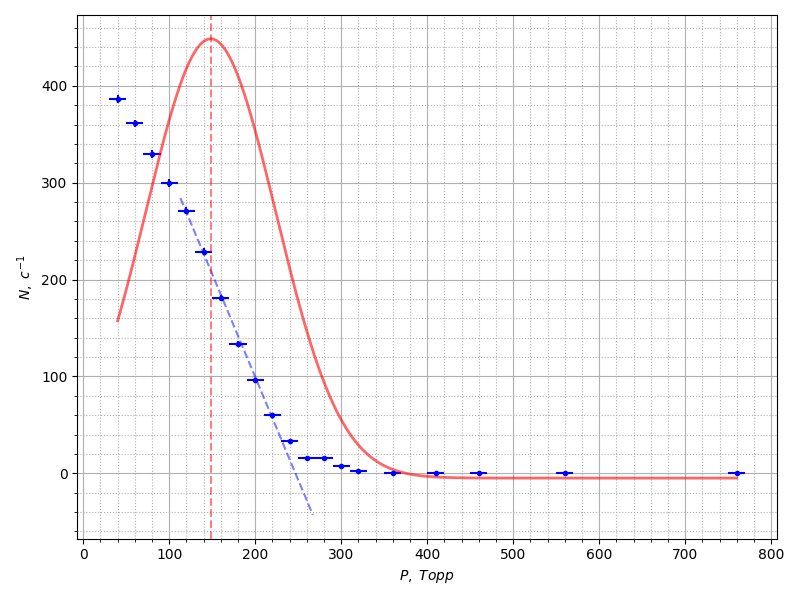
\includegraphics[width=0.9\linewidth]{5.4.1N(P).png}
			\caption{График зависимости $N(p)$}
    \end{figure}

	\subsection{ Определение пробега $\alpha$-частиц с помощью ионизационной камеры}
	


	
	\begin{enumerate}
		\item Проведем измерения зависимости тока от давления. Результаты запишем в таблицу \ref{AlphaParticles_I(P)}.
	

			% \caption{Зависимость тока от давления}
			% \label{AlphaParticles_I(P)}

	
	
		Построим график зависимости $I(P)$, по которому определим $P_\text{э}$ как пересечение двух прямых, продолженных на прямолинейных участках графика:
		\begin{equation*}
			P_\text{э} = (611 \pm 10) \text{ торр}.
		\end{equation*}
	
		При найденном давлении длина свободного пробега равна расстоянию между внутренним и внешним электродами:
		\begin{equation*}
			L = \frac{10-0,5}{2} \text{ см} = 4,75 \text{ см}.
		\end{equation*}
	
		Пересчитаем длину свободного пробега для нормальных условий:
		\begin{equation*}
			R_\text{э} = L\frac{P_\text{э}}{P_0}, \text{ где } P_0 = 760 \text{ торр}.
		\end{equation*}
		
		Тогда:
		\begin{equation*}
			R_\text{э} = (3,82 \pm 0,06) \text{ см}.
		\end{equation*}	
	
		\begin{equation*}
			R'_\text{э} = (4,47 \pm 0,07) \cdot 10^{-3} \;\dfrac{\text{г}}{\text{см}^2}.
		\end{equation*}		
	
		
		\begin{figure}[h!]
			\centering
			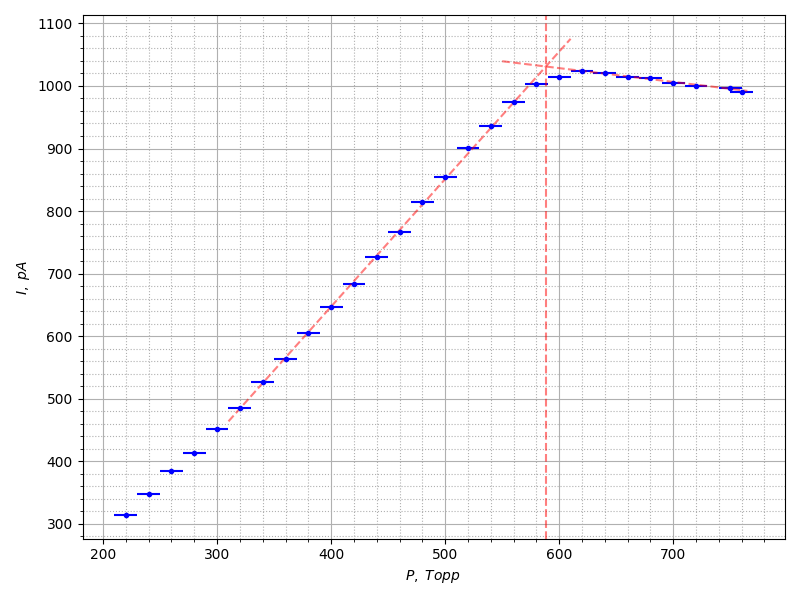
\includegraphics[width=\linewidth]{5.4.1I(P).png}
			\caption{Зависимость $I(P)$}
		\end{figure}
	
		Посчитаем энергию $\alpha$-частиц:
		\begin{equation*}
			\boxed{E = (5,22 \pm 0,05) \text{ МэВ}}
		\end{equation*}
	
		В этот раз значение чрезвычайно близко к истинному $E = 5,15$ МэВ.
	
	\end{enumerate}

	\newpage
\section{Обсуждение результатов и выводы.}
	
	\begin{table}[h!]
		\centering
		\resizebox{\columnwidth}{!}{%
			\begin{tabular}{c|c|c|c|}
				\cline{2-4}
				& Счетчик Гейгера & Сцинтилляционный счетчик & Ионизационная камера \\ \hline
				\multicolumn{1}{|c|}{$R_\text{э}$, см}                   & $1,9 \pm 0,3$   & $2,4 \pm 0,2$            & $3,82 \pm 0,06$      \\ \hline
				\multicolumn{1}{|c|}{$R_\text{ср}$, см}                  & $1,77 \pm 0,05$ & $1,32 \pm 0,05$          & --                   \\ \hline
				\multicolumn{1}{|c|}{$R'_\text{э}$, $10^{-3}$ г/см$^2$}  & $2,2 \pm 0,4$   & $2,8 \pm 0,2$            & $4,47 \pm 0,07$      \\ \hline
				\multicolumn{1}{|c|}{$R'_\text{ср}$, $10^{-3}$ г/см$^2$} & $2,07 \pm 0,06$ & $1,55 \pm 0,06$          & --                   \\ \hline
				\multicolumn{1}{|c|}{$E_\text{э}$, МэВ}                  & $3,3 \pm 0,4$   & $3,8 \pm 0,2$            & $5,22 \pm 0,05$      \\ \hline
				\multicolumn{1}{|c|}{$E_\text{ср}$, МэВ}                 & $3,13 \pm 0,06$ & $2,9 \pm 0,1$            & --                   \\ \hline
			\end{tabular}%
		}
	\end{table}
	
	В данной работе мы измерили пробег $\alpha$-частиц в воздухе. Получили достаточно много разных значений, неслабо отличающихся друг от друга. Однако они все оказываются одного порядка и даже того же порядка, что и истинное значение. Это же верно и для найденных энергий $\alpha$-частиц. Значения, найденные с помощью счетчика Гейгера и сцинтилляционного счетчика, занижены по сравнению с реальным значением. Лучше всего к действительности подобрался способ с ионизационной камерой: $E = (5,22 \pm 0,05)$ МэВ; в то время как настоящее значение $E = 5,15$ МэВ. Заниженные значения в первых двух методах объясняется несовершенством методики: $\alpha$-частицы тратят свою энергию на преодоление дополнительных препятствий. 
	
	
	


\end{document}
